\section{Implementation}

\subsection{Apps}
Bei Django ist es üblich, die Funktionalitäten in verschiedene Apps aufzuteilen. Eine App in Django ist vergleichbar mit einem Package in Java. Das Ziel ist es also, den Code so auf die verschiedenen Apps aufzuteilen, dass diese unabhängig voneinander wiederverwendet werden können. Aus diesem Grund wurde entschieden folgende Apps zu erstellen: \\
\newline
\begin{tabularx}{\textwidth}{| X | X |}
	\hline
		\textbf{Apps} & \textbf{Beschreibung} \\
	\hline
		Users & Die Users App soll alles was mit den Users zu tun hat verwalten. Also das erstellen und bearbeiten von Usern wie auch dem einloggen und ausloggen. \\
	\hline
		School admins & Die School admins App ist für die Zuweisung der Schüler und Lehrer an Klassen zuständig, sowie das erstellen von Klassen. \\
	\hline
		Exercises & Die Exercises App bietet die Logik an um Aufgaben zu definieren. \\
	\hline 
		Dashboards & Die Dashboards App ist dazu da, den Benutzern eine Übersicht zu bieten. \\
	\hline
		Forums & In der Forum App wird die komplette Logik für das Forum implementiert. \\
	\hline
		Study contents & Die Study contents App beinhaltet alles was mit dem bereitgestellten Inhalt zu tun hat. \\
	\hline
\end{tabularx} \\


\noindent Die Logik kann ohne Probleme in die verschiedenen Apps aufgeteilt werden. Das Problem dabei ist jedoch die Datenbank. In Django ist es best-practise, die benötigten Models (Datenbanktabellen) jeweils in der entsprechenden App zu implementieren. Da die einzelnen Tabellen aus der Datenbank eine starke Bindung zu den anderen Tabellen haben, geht diese Bindung somit auch auf die Apps über. Dadurch schwindet der Sinn, die Logik in verschiedene Apps aufzuteilen. Es gibt zwei Möglichkeiten, mit diesem Problem umzugehen. Die erste wäre es, alle Apps zu einer grossen zusammenzulegen und die zweite wäre es bei der zu Beginn gewählten Aufteilung zu bleiben und die starke Koppelung hinzunehmen. 

%TODO Weiterschreiben


\subsection{URLs}

\begin{table}[h]
	\centering
	\begin{tabu} to 0.9\textwidth {X X X}
	\toprule
		\textbf{URL} & \textbf{View} & \textbf{Template} \\
	\bottomrule
		/ & SubjectListView & subject\_list.html \\
	\bottomrule
		\textbf{user/} \\
		login/ & LoginView & registration/login.html \\
		logout/ & LogoutView & registration/logged\_out.html \\ 
		profile/ & ProfileUpdateView & user/profile.html \\
		<type>/create/ & UserCreateView & user/user\_form.html \\ 
		<pk>/update/ & UserUpdateView & user/user\_form.html \\
		<pk>/delete/ & UserDeleteView & user/user\_confirm\_delete.html \\
		
		\textbf{subject/} \\
		<subject>/ & TopicListView & study\_content/topic\_list.html \\
		<subject>/<topic>/ & LessonListView & study\_content/lesson\_list.html \\
		<subject>/<topic>/<pk>/ & LessonDetailView & study\_content/lesson\_detail.html \\
		
		\textbf{school\_admin/} \\
		/ & ClassUserListView & school\_admin/admin\_overview.html \\
		class/create/ & ClassCreateView & school\_admin/class\_create.html \\
		class/<class\_pk>/update/ & ClassUpdateView & school\_admin/admin\_class\_management.html \\
		class/<class\_pk>/delete/ & ClassDeleteView & school\_admin/class\_confirm\_delete.html \\
		
		\textbf{exercise/} \\
		%TODO
		
		\textbf{statistic/} \\
		/ & StatisticListView & statistic/statistic\_subject.html \\
		exercise/<topic>/<class\_id>/ & StatisticExerciseListView & statistic/statistic\_exercise.html \\
		exercise/<topic>/<exercise>/<class\_id>/ & StatisticDetailView & statistic/statistic\_detail.html \\
		ajax/load\_subjects/ & & subject\_dropdown\_list\_options.html \\
		ajax/load\_data/ & & subject\_load\_data.html \\
		
		\textbf{error/} \\
	\end{tabu}
	\captionof{table}{URLs}
\end{table}


Django bietet eine simple Möglichkeit an, um zu definieren, welche Seite mit welcher URL aufgerufen werden kann. Wie man im Bild unten sehen kann, wird eine URL in drei, jeweils kommaseparierten, Teilen definiert:

\begin{minipage}{\textwidth}
	\begin{figure}[H]
		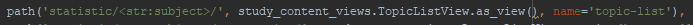
\includegraphics[width=\textwidth, height=\textheight, keepaspectratio]{images/URLBsp.png}
		\caption{URL definition}
	\end{figure}
\end{minipage}


\begin{itemize}
	\itemsep0em
	\item Pfad \\
	Der erste Teil ist der Pfad. Im Beispiel wird der Pfad 'statistic/<str:subject>/' definiert. Das bedeutet, die entsprechende Seite soll über den Pfad ''statistic/'' gefolgt von einem beliebigen Text, in unserem Fall der Titel eines Subjects (zB. Mathematik, Deutsch, etc.), erreichbar sein. 
	\item View \\
	Mit dem zweiten Teil wird definiert, welche View angezeigt werden soll. Im Bild ist es zwar nicht ersichtlich, jedoch werden die Views aus der aktuellen App importiert und können über den Namen ''study\_content\_views'' angesprochen werden. Anschliessend kann über diesen Namen die View angespochen werden, die dargestellt werden soll. In unserem Fall ist dies die View ''TopicListView''.
	\item Name \\
	Im dritten und letzten Teil wird der Pfaddefinition einen Namen gegeben. Dieser Name muss über die ganze Applikation hinweg eindeutig sein und kann dazu verwendet werden, Verlinkungen zwischen den einzelnen Seiten zu definieren. Der Vorteil dabei ist, dass der Pfad sich ändern kann, ohne dass die gemachten Verlinkungen angepasst werden müssen.
\end{itemize}


\noindent Es können beliebig viele solcher URLs definiert werden. Das Framework schreibt keine klare Struktur vor. Aus diesem Grund haben wir uns dazu entschieden, die URL Definitionen auf mehere Dateien aufzuteilen und jeweils direkt in den einzlenen Apps abzulegen. Mit diesem Schritt erreicht man mehrere Vorteile. Zum einen wird das Definieren der URLs einiges übersichtlicher und einfacher anzupassen und zum anderen kann man das Risiko von Konflikten zwischen den URLs reduzieren. Schauen wir uns das ganze anhand eines Beispiels an. \\
\begin{minipage}{\textwidth}
	\begin{figure}[H]
		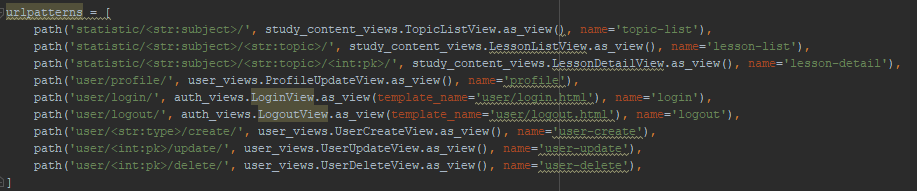
\includegraphics[width=\textwidth, height=\textheight, keepaspectratio]{images/URLschlecht.png}
		\caption{URL Beispiel}
	\end{figure}
\end{minipage}

\noindent Im Bild oben sieht man eine kleine Sammlung verschiedener URLs. Bei genauerer Betrachtung fällt auf, dass die URLs von zwei verschiedenen Apps stammen. Die ersten drei URLs gehören zu den Statistiken und die nachfolgenden zur Benutzerverwaltung. Natürlich kann man Vorkehrungen treffen um das ganze übersichtlicher darzustellen, jedoch wird es schwieriger je mehr Definitionen vorliegen. Zum weiteren ist es sehr aufwendig, wenn die URLs angepasst werden sollen. Sollten zum Beispiel die URLs von ''user/...'' auf ''benutzer/...'' geändert werden, muss dies manuell überall angepasst werden. 
Mit unserer Lösung wird diese Datei in drei neue Dateien aufgeteilt und ist danach folgendermassen strukturiert: \\

\noindent \textbf{user/urls.py} \\
Diese Datei wird in der App ''user'' abgelegt und kann so zusammen mit der App simpel in eine andere Applikation kopiert und verwendet werden. Im Bild unten werden nun die URLs dargestellt, welche zur Benutzerverwaltung gehören und man kann erkennen, dass die URLs kürzer geworden sind. Das führende ''user/'' wurde entfernt. Wieso das möglich und auch gewünscht ist, wird weiter unten beschrieben. \\
\begin{minipage}{\textwidth}
	\begin{figure}[H]
		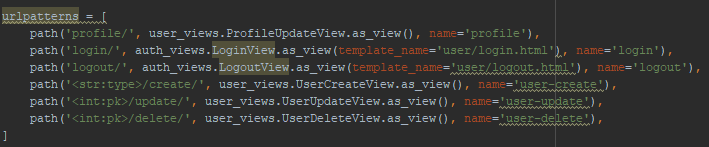
\includegraphics[width=\textwidth, height=\textheight, keepaspectratio]{images/URLuser.png}
		\caption{URL user}
	\end{figure}
\end{minipage}


\noindent \textbf{statistic/urls.py} \\
Diese Datei wird in der App ''statistic'' abgelegt. Wie oben das führende ''user/'' entfernt wurde, konnte auch hier auf das führende ''statistic/'' verzichtet werden. \\
\begin{minipage}{\textwidth}
	\begin{figure}[H]
		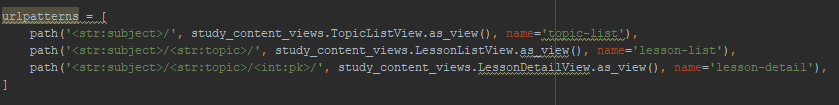
\includegraphics[width=\textwidth, height=\textheight, keepaspectratio]{images/URLstatistic.png}
		\caption{URL statistic}
	\end{figure}
\end{minipage}


\noindent \textbf{urls.py} \\
Diese Datei befindet sich in keiner eigenen App, sondern liegt global in der Applikation. Der Inhalt der Datei unterscheidet sich auch gegenüber den andereren Dateien. Hier werden keine URLs definiert, sondern es wird angegeben, wo die definierten URLs abgelegt sind. Oben wurde erwähnt, dass die führenden Pfadelemente (''user/'' und ''statistic/'') weggelassen wurden. Effektiv wurden sie jedoch hierhin verschoben. Sollen nun die URLs der Benutzerverwaltung von ''user/...'' nach ''benutzer/...'' geändert werden, kann dies hier vorgenommen werden und wirkt sich auf alle URLs in der Datei ''user/urls.py'' aus. Nun ist es auch möglich in verschiedenen Apps die selben URLs zu definieren, da sie hier beim einbinden mit dem führenden Pfadelement voneinander unterschieden werden können. Dies kann hilfreich sein, wenn Apps von anderen Entwicklern eingebaut werden würden. \\
\begin{minipage}{\textwidth}
	\begin{figure}[H]
		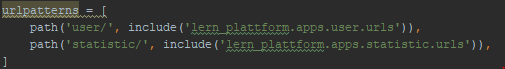
\includegraphics[width=\textwidth, height=\textheight, keepaspectratio]{images/URLglobal.png}
		\caption{URL}
	\end{figure}
\end{minipage}




\subsection{Testing}

\subsection{Allgemein}
Das Testen einer Webseite ist eine komplexe Aufgabe, da eine Webseite aus mehreren Schichten unterschiedlicher Logik aufgebaut ist. Das geht von HTTP-Requests über die Validierung von Formularen bis hin zum Rendern von Templates. Mit dem Django-Test-Framework ist es möglich, HTTP-Requests zu simulieren, Testdaten einzufügen, den Output der Applikation zu inspizieren und im allgmeinen zu prüfen, dass der geschriebene Code das tut, was er tun soll.

\subsection{Datenbank}
Damit die Tests nicht von bereits vorhanden Daten in der Datenbank beeinflusst werden, wird für jeden Testdurchlauf eine eigene temporäre Datenbank erstellt, die exakt wie die in der Produktion verwendete Datenbank konfiguriert ist. Diese temporäre Datenbank wird nach der Testdurchführung wieder vom System entfernt.

\subsection{Test Client}
Der Test-Client ist eine Pythonklasse, welche als einfacher Webbrowser dient. Mit ihm kann man auf Applikationsebene mit den erstellten Django-Apps agieren. Das heisst, man kann gut und einfach GET und POST Requests simulieren und kann den Inhalt der Webseite überprüfen. 